\documentclass{article}

\usepackage{shyne}

% document format
\topmargin 0in
\oddsidemargin 0in
\evensidemargin 0in
\headheight 0in
\headsep 0in
\topskip 0in
\textheight 9in
\textwidth 6.5in
\linespread{1.3}

\begin{document}

\begin{flushleft}
\section*{Group Work - Week 6}
\paragraph{1} The best player on the Metro State basketball team successfully makes 85\% of her free throws. During a typical game she attempts 15 free throws. (If she attempts a different number of free throws, it is not a typical game.)
\begin{enumalpha}
\item Is the number of free throws she makes in a typical game a proper binomial random variable? What are the values of $n$, $p$ and $q$?\\
\medskip
\bt{Yes. All the requirements are met...}
\begin{itemize}
\item \bt{The distribution must represent a fixed number of trials (because we define a ``typical" game as one where she attempts 15 free throws, we have a fixed number of trials)}
\item \bt{Each trial must have exactly two possible outcomes (free throw made / not made)}
\item \bt{Each trial must be independent of the other trials (if you ignore the phenomenon of ``streaks", which seem to have no statistical support)}
\item \bt{Each trial must have the same probability for success (again, you might need to ignore the effect of fatigue or other influences over the course of the game. In practice, one assumes those kinds of effects average out over time.)}
\end{itemize}
\medskip
$\bv{n=15, \qquad p = 0.85, \qquad q = 1- p = 0.15}$

\vspace{0.5in}


\item What is the expected number of free throws made per game? What is the standard deviation?\\
\medskip
$\bv{\E(X) = \mu = np = 15 \times 0.85 = 12.75}$\\
\smallskip
$\bv{\sigma = \sqrt{npq} = \sqrt{15 \times 0.85 \times 0.15} = \sqrt{1.9125} \approx 1.383}$

\vspace{0.5in}

\newpage
\item What is the probability she makes all her free throws in a typical game? Is that unusual? What is the probability she makes at least 12 free throws? Less than 12?\\
\medskip
$\bv{P(X=15) = 0.087 >0.05}$\bt{, not unusual}\\ 
\smallskip
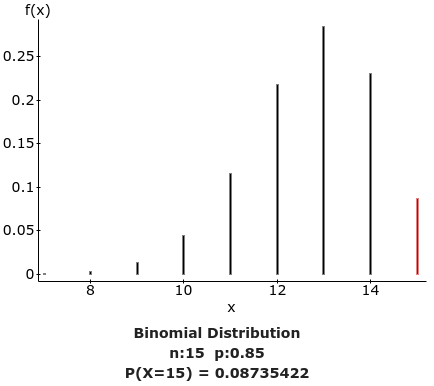
\includegraphics[width=2.5in]{images/group06_Q1_c_1}\\
\bigskip
$\bv{P(X \ge 12) = 0.823}$\\
\smallskip
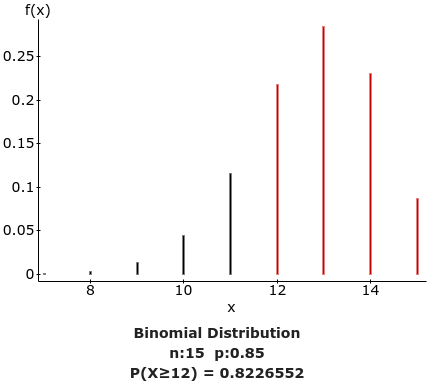
\includegraphics[width=2.5in]{images/group06_Q1_c_2}\\
\bigskip
$\bv{P(X < 12) = 0.177}$\\
\smallskip
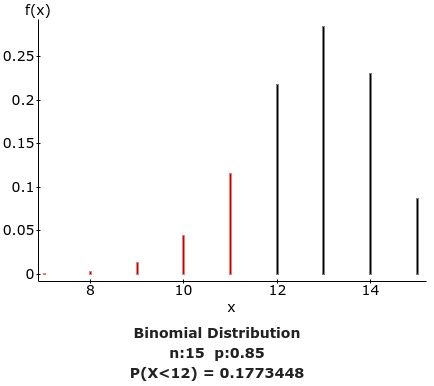
\includegraphics[width=2.5in]{images/group06_Q1_c_3}\\

\vspace{0.5in}

\newpage
\item What are unusual numbers of free throws made per game?\\
\medskip
\bt{Unusual values: }$\bv{\mu \pm 2 \sigma}$\\
\medskip
$\bv{\mu - 2\sigma = 12.75 - 2\times 1.383 = 9.984}$\\
\bt{Anything less than 9.984 would be an unusually/significantly low number of free throws to make. Since free throws made is a discrete variable, 9 or less made free throws are unusually low.}\\
\medskip
$\bv{\mu - 2\sigma = 12.75 + 2\times 1.383 = 15.516}$\\
\bt{Similarly, 16 or more free throws made would be unusually high, but since it is not possible to make 16 out of 15 free throws, there is no unusually high number of free throws made.}

\end{enumalpha}

\newpage

\paragraph{2} Eleanor is taking two classes, statistics and ethics. After the midterm exams, Eleanor got 86 on her statistics midterm and she scored better than 88\% of the class on her ethics midterm. The statistics midterm scores were approximately normally distributed with a mean of 84 and a standard deviation of 5.2. The ethics midterm scores were approximately normally distributed with a mean of 71.5 and a standard deviation of 9.8. 

\begin{enumalpha}
\item What is the probability a randomly selected student did worse than Eleanor on the statistics midterm? That is, what is $P(X < 86)$? Or, what percentile is Eleanor's statistics grade?\\
\medskip
$\bv{P(X < 86) = 0.650}$\\
\smallskip
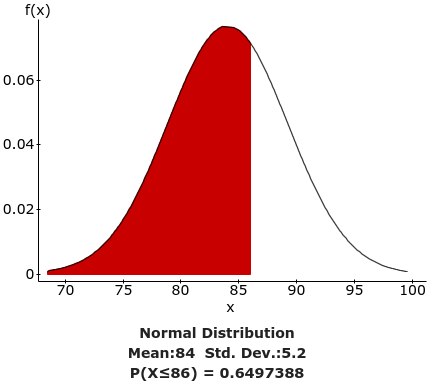
\includegraphics[width=2.5in]{images/group06_Q2_a}\\

\vspace{0.25in}
\item What score did Eleanor get on her ethics midterm? That is, for what $x$ is $P(X < x) = 0.88$? \\
\medskip
\bt{Eleanor got an 83 on the ethics midterm... }$\bv{P(X < 83) = 0.88}$\\
\smallskip
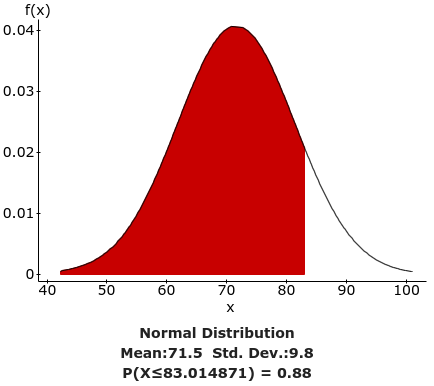
\includegraphics[width=2.5in]{images/group06_Q2_b}\\

\vspace{0.25in}
\item Calculate the z-scores for Eleanor's two midterm grades. In which class did she do better?\\
\medskip
$\ds \bv{z_{stat} = \frac{x - \mu_{stat}}{\sigma_{stat}} = \frac{86 - 84}{5.2} = 0.385}$\\
\medskip
$\ds \bv{z_{eth} = \frac{x - \mu_{eth}}{\sigma_{eth}} = \frac{83 - 71.5}{9.8} = 1.173}$\\
\medskip
\bt{Eleanor did better on her ethics midterm.}


\end{enumalpha}

\end{flushleft}
\end{document}